\documentclass{report}
\usepackage{setspace}
%\usepackage{subfigure}

% my extra package imports;
\usepackage{caption}
\usepackage{float}
\usepackage{hyperref}
\usepackage{subcaption}
\usepackage{graphicx}
\usepackage{graphics}
\usepackage{tikz}
\usetikzlibrary {positioning, shapes, bayesnet}
\graphicspath{{./}}
\usepackage{natbib}
% end of my imports;

\pagestyle{plain}
\usepackage{amssymb,color}
\usepackage{amsfonts}
\usepackage{latexsym}
\usepackage{a4wide}
\usepackage{amsmath}

\newtheorem{theorem}{THEOREM}
\newtheorem{lemma}[theorem]{LEMMA}
\newtheorem{corollary}[theorem]{COROLLARY}
\newtheorem{proposition}[theorem]{PROPOSITION}
\newtheorem{remark}[theorem]{REMARK}
\newtheorem{definition}[theorem]{DEFINITION}
\newtheorem{fact}[theorem]{FACT}

\newtheorem{problem}[theorem]{PROBLEM}
\newtheorem{exercise}[theorem]{EXERCISE}
\def \set#1{\{#1\} }

\newenvironment{proof}{
PROOF:
\begin{quotation}}{
$\Box$ \end{quotation}}



\newcommand{\nats}{\mbox{\( \mathbb N \)}}
% \newcommand{\rat}{\mbox{\(\mathbb Q\)}}
\newcommand{\rats}{\mbox{\(\mathbb Q\)}}
\newcommand{\reals}{\mbox{\(\mathbb R\)}}
\newcommand{\ints}{\mbox{\(\mathbb Z\)}}

%%%%%%%%%%%%%%%%%%%%%%%%%%

% COVER PAGE;
\title{
  { \includegraphics[scale=.5]{ucl_logo.png}}\\
  {{\Huge Graph style transfer via Inverse Reinforcement Learning}}\\
  {\large An application to subway networks}\\
}

\date{Submission date: Day Month Year}
\author{
  Candidate Number: YLLK3\thanks{
      {\bf Disclaimer:}
      This report is submitted as part requirement 
      for the MSc Machine Learning at UCL. It is
      substantially the result of my own work except 
      where explicitly indicated in the text.
      The report may be freely copied and 
      distributed provided the source is explicitly acknowledged.
    }
    \\ \\
  MSc Machine Learning\\ \\
  Supervisor's name
}

\numberwithin{equation}{section}
\numberwithin{figure}{section}
\numberwithin{table}{section}  

%%%%%%%%%%%%%%%%%%%%%%%%%%%%%%%%%%%%%%%%%%%%%%%%%%%%%%%%%%%%%%%%%%
% START DOCUMENT;
\begin{document}
\onehalfspacing
\maketitle

%%%%%%%%%%%%%%%%%%%%%%%%%%%%%%%%%%%%%%%%%%%%%%%%%%%%%%%%%%%%%%%%%%
% ABSTRACT;
\begin{abstract}
  Summarise your report concisely.
\end{abstract}
\tableofcontents
\setcounter{page}{1}

%%%%%%%%%%%%%%%%%%%%%%%%%%%%%%%%%%%%%%%%%%%%%%%%%%%%%%%%%%%%%%%%%%
% NEW CHAPTER - INTRODUCTION;
\chapter{Introduction}

%%%%%%%%%%%%%%%%%%%%%%%%%%%%%%%%%%%%%%%%%%%%%%%%%%%%%%%%%%%%%%%%%%
% NEW CHAPTER - RL BACKGROUND;
\chapter{Reinforcement Learning Background}
\label{chap:RL}

\section{The Goal of Reinforcement Learning}
\label{sec:RLGoal}

The goal of Reinforcement learning is to learn a behaviour that 
optimises some reward signal. The key assumption is that 
any goal (be it high-level or otherwise) can be fomulated as 
maximisation of the reward signal.

In the Reinforcement learning setup, we distinguish between two 
key entities - environment and agent. The environment is the 
entity that specifies a set of rules based on which, an action 
is judged given its current configuration. 
More specifically, let the configuration or state of the 
environment at time $t$ be denoted by $s_t$. Then, 
given an action, $a_t$ at time $t$, the environment evaluates 
how good this action is, given its 
current state, and outputs a (scalar) reward signal (or reward), 
$r_{t+1}$, and also updates its state to $s_{t+1}$. The agent 
is the entity responsible for giving an action $a_t$. 

It is worth noting that there are 
different conventions about indexing the reward, but in this work 
we adopt the convention from the Sutton and Barto book 
\citep{Sutton1998} where the reward is thought of as feedback 
given to the agent the step after the action was taken.

The agent may not always have access 
to the environment's state and can maintain its own state, based 
on which it takes an action. We refer to such settings as partially 
observed problems. 

An example of such a problem could be a robot 
whose goal is to find its way out of a maze as quickly as possible.
Suppose the robot only `sees' what is 
immediately surrounding it, in which case this would be its state 
or observation, $o_t$. 
In contrast, if it had access to the environment's state, it could 
see the shortest path out of the maze and take the necessary actions 
that yield the greatest accumulated reward (or return).

\section{Markov Decision Process (MDP)}
\label{sec:RLMDP}
Based on the robot and maze example, the reader may have noticed 
that given the current state of the environment and an action taken 
by the robot, the next environment state does not depend on any 
past states and/or actions. That is, the environment state 
is first-order Markovian (given the present state and action). Indeed, this leads us to a convenint 
mathematical formulation of the dynamics of the 
Reinforcement learning problem called 
a Markov Decision Process (MDP).

An MDP is defined by the tuple 
($\mathcal{S},\; \mathcal{A},\; \mathcal{P},\; r(\cdot),\; \gamma$), where
\begin{itemize}
  \item $\mathcal{S}$ is the state space of the environment 
    (Markovian states).
  \item $\mathcal{A}$ is the action space (actions among which 
    the agent can select).
  \item $\mathcal{P}:\mathcal{S}\times \mathcal{A}\rightarrow\mathcal{S}$ 
    is the transition operator and specifies the transition 
    dynamics from 
    the current state-action pair to the next state.
  \item $r(\cdot)$ is the scalar-valued reward function 
    (usually defined as $r:\mathcal{S}\times \mathcal{A}\rightarrow \reals$, 
    although $r:\mathcal{S}\rightarrow \reals$ is also possible).
  \item $\gamma\in [0, 1]$ is the discount factor of rewards, which controls 
    how long or short sighted our objective is.
\end{itemize} 

The way $\gamma$ is used is typically alongside some function of 
the rewards collected along a path/trajectory. Let $\tau$ denote a 
path/trajectory given by:
\begin{equation}
  \tau:=(s_1, a_1, r_2, s_2, a_2, \ldots, s_T, a_T, r_{T+1}, s_{T+1}),\label{eq:tau} 
\end{equation} 
and $G:\mathcal{T}\rightarrow \reals$ denote the return 
function. Among the simplest examples of $G$ is the Monte-Carlo 
return:
\begin{equation}
  G(\tau):=\sum_{k=0}^{T-t}\gamma^kr_{t+k+1}.\label{eq:MCReturn}
\end{equation}
Looking at \eqref{eq:MCReturn}, we see that if we set $\gamma=0$ 
this corresponds to a myopic return, $G_t=r_{t+1}$, while if 
$\gamma=1$, we get a far-sighted return where we equally weigh 
all rewards along the trajectory $\tau$.

The MDP as currently defined induces a probabilistic graphical model 
(pgm) that is illustrated in Figure \ref{fig:MDP}.

\begin{figure}[H]
  \centering
  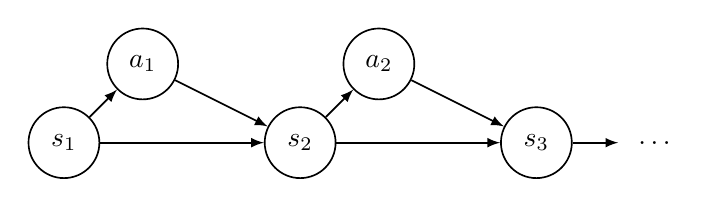
\begin{tikzpicture}[-latex ,auto ,node distance =1 cm and 1cm ,
      on grid , inner sep=0pt, minimum size=9mm,
      semithick, state/.style={circle, draw}]
      % s1, a1, s2;
      \node[state](s_1) at(0,0) {$s_1$};
      \node[state](a_1) at(1,1) {$a_1$};                                                                                                       
      \path (s_1) edge (a_1);
      \node[state](s_2) at(3,0) {$s_2$};
      \path (s_1) edge (s_2);
      \path (a_1) edge (s_2);
      % s2, a2, s3
      \node[state] (a_2) at(4,1) {$a_2$};
      \path (s_2) edge (a_2);
      \node[state] (s_3) at(6,0){$s_3$};
      \path (s_2) edge (s_3);
      \path (a_2) edge (s_3);
      % dots;
      \node (dots) at(7.5,0) {$\ldots$};
      \path (s_3) edge (dots);
  \end{tikzpicture}
  \caption{\label{fig:MDP} Graph of MDP.}
\end{figure}





\begin{itemize}
  \item Define the RL objective - optimising long term reward 
    or the episodic objective with the returns;
  \item Give the Bellman equations as a means to solve an MDP;
    Give proof of the convergence of those Bellman operators;
  \item Make the claim about the existence of an optimal greedy 
    policy, given an MDP;
\end{itemize}

%%%%%%%%%%%%%%%%%%%%%%%%%%%%%%%%%%%%%%%%%%%%%%%%%%%%%%%%%%%%%%%%%%
% NEW CHAPTHER - IRL THEORY;
\chapter{Inverse Reinforcement Learning}
Test citation \citep{NgIRL} - done.
\begin{itemize}
  \item State the goal of IRL - estimate an objective function
    that when optimised should yield a behaviour similar to the 
    one in the demos by the expert.
  \item Argue the point about the ill-posedness of IRL, which makes 
    classic optimal control not suitable for the job.
  \item Talk about the max-margin approach (Ng) to IRL.
    State drawbacks;
  \item Talk about the max-entropy Ziebart approach;
    Show the (soft) `duality' between this probabilistic setting and 
    the updates from the Bellman equations - see Levine lectures 
    and motivations and his review paper. Here should talk about the 
    works of Todorov, Sergey's review paper and SAC as a means to 
    work in this probabilistic setting.
\end{itemize}

%%%%%%%%%%%%%%%%%%%%%%%%%%%%%%%%%%%%%%%%%%%%%%%%%%%%%%%%%%%%%%%%%%
% NEW CHAPTER - GRAPH REPRESENTATIONS;
\chapter{Graph representations}
\begin{itemize}
  \item Give a lit review with the Scarsalli (can be enough to just 
  mention his name and give the general MPNN structure).
  \item Talk about the applications of GNNs - e.g., the Kipf paper 
    with GCN and application to citation graphs;
  \item Talk about the GATv2 which I am using.
  \item Read/skim the new paper about how much can gnns learn.
  \item State drawbacks and potential reasons, why it is difficult 
    to work with graph topography rather than topology when using 
    GNNs.
\end{itemize}

%%%%%%%%%%%%%%%%%%%%%%%%%%%%%%%%%%%%%%%%%%%%%%%%%%%%%%%%%%%%%%%%%%
% NEW CHAPTER - OUR CONTRIBUTION;
\chapter{Our Contribution}
\begin{itemize}
  \item Basically the different spins on GrphOpt;
    \subitem Check effect of adding separate reward encoder;
    \subitem Check effect of UT trick - didn't seem so good, might drop;
    \subitem Check effect of multitask training - see if works;
    \subitem Talk about particular implementation experience
      gathering and storing it in the Replay Buffer; talk about 
      the batch-sampling time reward computation and not wasting 
      state-action trajectory experience by having to clear the 
      buffer after reward update, had we stayed with vanilla description;
\end{itemize}

%%%%%%%%%%%%%%%%%%%%%%%%%%%%%%%%%%%%%%%%%%%%%%%%%%%%%%%%%%%%%%%%%%
% NEW CHAPTER - EXPERIMENTS;
\chapter{Experiments}
\begin{itemize}
  \item T1 is about transferring learned reward on target graph;
  also compares learned policy directly on target, compared to 
  training new policy on target with frozen reward;
  \item T2 is about MRR - based on top 25 proposal edges;;
  \item T3 is about running learned policy on source graph and 
  seeing if we get similar graphs;
  \item I also get rewards along paths.
  \begin{itemize}
    \item Compare convergence rate of eval returns over seeds
      and comment on speed;
  \end{itemize}
  \item BA40 to BA80 - 10 seeds
  \begin{itemize}
    \item GOptEpWeights, GOptPerDec, 
      GOptRewEncEpWeights, GOptRewEncPerDec,
    \item THIS IS NOT APPLICABLE TO BA GRAPHS - ONLY TRY IT ON GRAPHS 
      WITH MEANINGFUL TOPOGRAPHY!!! - Then take better of EpWeights and PerDec and do 
      GOptMultitaskBetterWeight and GOptRewEncMultitaskBetterWeight,
    \item also run UT trick with the better weight setting;
  \end{itemize}
    
  \item T1 and T3 run together - this is $10\times 8=80$ experiments;
  \item T2 runs alone - this is $10\times 8=80$ experiments;
  \item total is 160 experiments;
  \item  Run best config on Urban nets 10 times;
\end{itemize}
\chapter{Conclusion and Further work}


\chapter{title of first chapter}
This is just a bare minimum to get started.  There is unlimited guidance on using latex, e.g. {\tt https://en.wikibooks.org/wiki/LaTeX}.   You are still responsible to check the detailed requirements of a project, including formatting instructions, see \\
{\tt https://moodle.ucl.ac.uk/pluginfile.php/3591429/mod\_resource/content/7/UGProjects2017.pdf}.
Leave at least a line of white space when you want to start a new paragraph.

Mathematical expressions are placed inline between dollar signs, e.g. $\sqrt 2, \sum_{i=0}^nf(i)$, or in display mode
\[ e^{i\pi}=-1\] and another way, this time with labels,
\begin{align}
\label{line1} A=B\wedge B=C&\rightarrow A=C\\
&\rightarrow C=A\\
\intertext{note that}
n!&=\prod_{1\leq i\leq n}i \\
\int_{x=1}^y \frac 1 x \mathrm{d}x&=\log y
\end{align}
We can refer to labels like this \eqref{line1}.   

\chapter{title of second chapter}
% Often lots of citations here (and elsewhere), e.g. \cite{Rey:D} or \cite[Theorem 2.3]{PriorNOP70}.   Bibtex can help with this, but is not essential. If you want pictures, try

\begin{center}
\includegraphics[scale=.5]{aristotle.jpg}
\end{center}
You can use 
\begin{itemize}
\item lists
\item like this
\end{itemize}
or numbered
\begin{enumerate}
\item like this,
\item or this
\end{enumerate}
but don't overdo it.
\chapter{title of third chapter}
If you have a formal theorem you might try this.
\begin{definition}\label{def}
See definition~\ref{def}.
\end{definition}
\begin{theorem}
For all $n\in\nats,\; 1^n=1$.
\end{theorem}
\begin{proof}
By induction over $n$.
\end{proof}

\chapter{etc.}
\appendix

\bibliographystyle{apa}
\bibliography{my_bib.bib}

% \begin{thebibliography}{HHM99}


% \bibitem[Pri70]{PriorNOP70}  %%only an example
% A.~Prior.
% \newblock The notion of the present.
% \newblock {\em Studium Generale}, 23:  245--248, 1970.


% \bibitem[Rey97]{Rey:D}
% M.~Reynolds.
% \newblock A decidable temporal logic of parallelism.
% \newblock {\em Notre Dame Journal of Formal Logic}, 38(3):  419--436,
%   1997.
% \end{thebibliography}
% \chapter{Other appendices, e.g. code listing}

\end{document}